\documentclass[12pt]{article}
\usepackage{geometry}                % See geometry.pdf to learn the layout options. There are lots.
\geometry{letterpaper}                   % ... or a4paper or a5paper or ... 
%\geometry{landscape}                % Activate for for rotated page geometry
\usepackage[parfill]{parskip}    % Activate to begin paragraphs with an empty line rather than an indent
\usepackage{graphicx}
\usepackage{amssymb}
\usepackage{subfig}
\usepackage{verbatim}
\usepackage{fullpage}
\usepackage{pstricks,pst-node,pst-tree}



\title{Breakpoints for farm field runoff}
\author{Wesley Brooks}
\date{}                                           % Activate to display a given date or no date

\usepackage{Sweave}
\begin{document}
\setkeys{Gin}{width=0.9\textwidth}    %make figures a bit wider than the Sweave default.
\maketitle

First read the data:
\vspace{3mm}

\begin{Schunk}
\begin{Soutput}
[1] 831
\end{Soutput}
\end{Schunk}

\vspace{5mm}

The following is the R function that produces a piecewise regression model:


\newpage

And the next function (\verb+peicewise_plot+) plots the piecewise regression model:


\newpage
We identify the best breakpoint by using R's optimize function to minimize the residual standard error:

\begin{Schunk}
\begin{Sinput}
> #soil_moisture_limits = c(33, 43) #set the limits
> #optimize(piecewise, soil_moisture_limits, x=data$sm, y=data$rc)$minimum
\end{Sinput}
\end{Schunk}



\vspace{5mm}
Now, let us do the soil moisture breakpoint analysis. The breakpoints at each farm individually, and for all farms in aggregate are found by the following code (breakpoints are stored in the variable \verb+sm_breakpoints+ for use in plotting [next code chunk]):\\


\begin{Schunk}
\begin{Soutput}
Breakpoints by farm:
\end{Soutput}
\begin{Soutput}
df1: 35
df3: 35
df5: 40
df7: 40
df8: 40
koepke: 35
pagel: 35
saxon: 40
\end{Soutput}
\end{Schunk}

\newpage
Then the plots are produced by calling the function \verb+piecewise_plot+ (code is listed above):\\



\begin{figure}
    \begin{center}
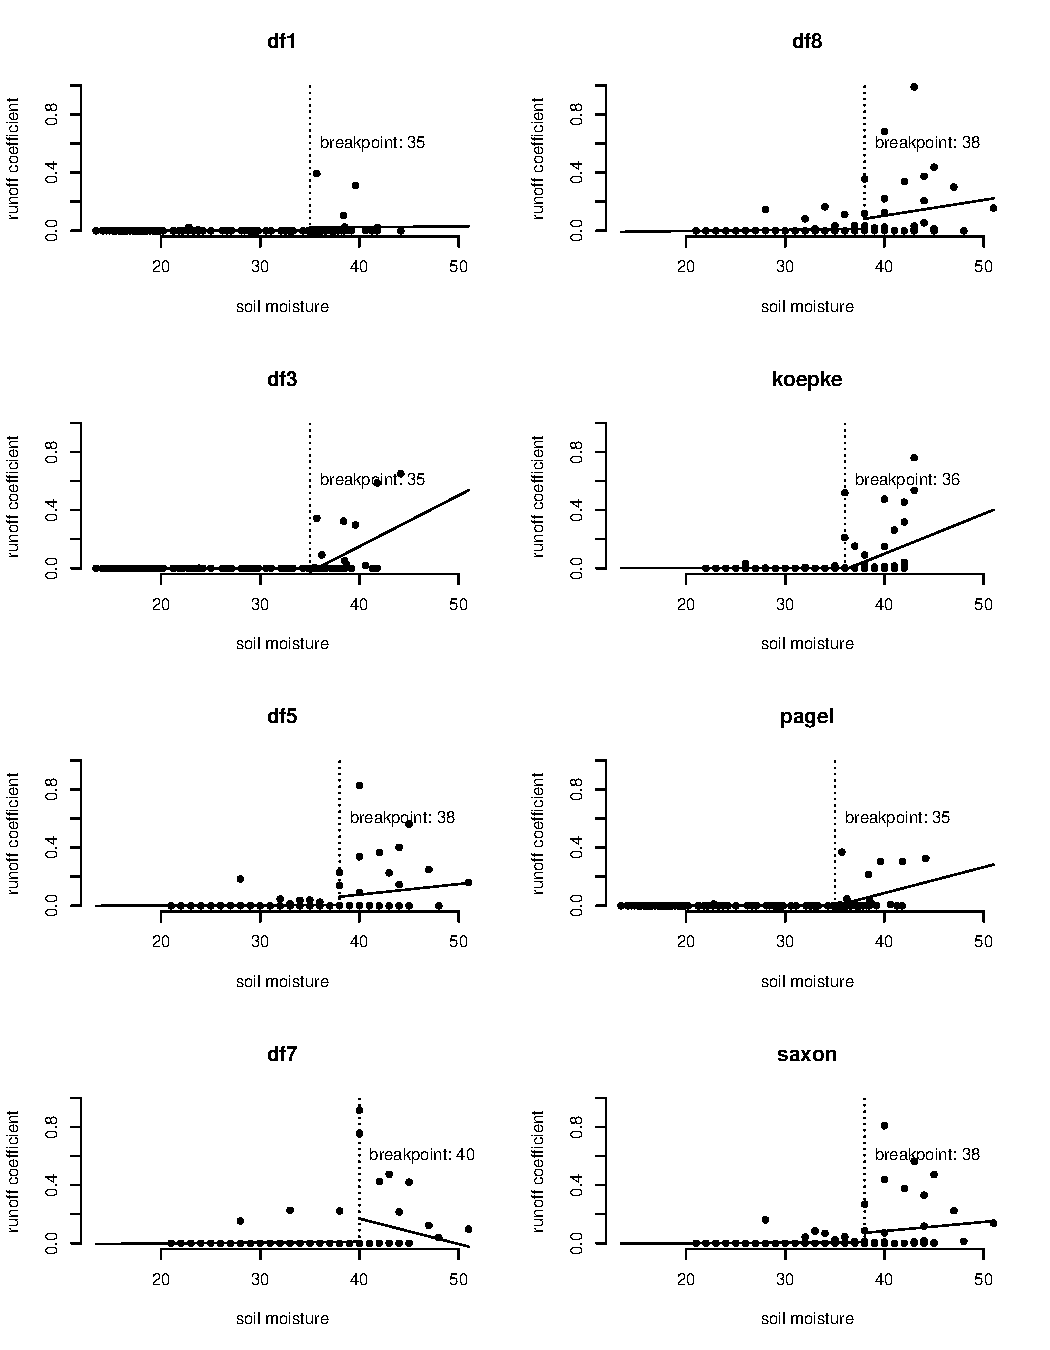
\includegraphics{runoff-sm}
    \end{center}
    \caption{caption.\label{sm}}
\end{figure}


Now get the I30 breakpoints:\\

\begin{Schunk}
\begin{Soutput}
df1: 2.3
df3: 0.7
df5: 2.2
df7: 2.1
df8: 3.4
koepke: 1.5
pagel: 2.3
saxon: 2.1
\end{Soutput}
\end{Schunk}


When we put the events in bins based on their antecedent soil moisture (SM: high, medium, and low), the following are the I30 breakpoints (units are centimeters of rain per hour):\\

\begin{Schunk}
\begin{Soutput}
Intensity breakpoints at koepke when binned by soil moisture:
0 <= SM < 30: 3.3
30 <= SM < 35: 1.8
35 <= SM < Inf: 1.6

Intensity breakpoints at pagel when binned by soil moisture:
0 <= SM < 30: 1.3
30 <= SM < 35: 0.6
35 <= SM < Inf: 0.6

Intensity breakpoints at saxon when binned by soil moisture:
0 <= SM < 35: 1.8
35 <= SM < 40: 1.2
40 <= SM < Inf: 2
\end{Soutput}
\end{Schunk}



\begin{figure}
    \begin{center}
\includegraphics{runoff-I30_binned}
    \end{center}
    \caption{Top row: Koepke, middle row: Pagel, bottom row: Saxon.\label{I30_binned}}
\end{figure}


When we put the events in bins based on their antecedent soil moisture (SM: high, medium, and low), the following are the precipitation breakpoints (units are centimeters of rain):\\

\begin{Schunk}
\begin{Soutput}
Precipitation breakpoints at koepke when binned by soil moisture:
0 <= SM < 30: 2.8
30 <= SM < 35: 1.72
35 <= SM < Inf: 1.58

Precipitation breakpoints at pagel when binned by soil moisture:
0 <= SM < 30: 2.63
30 <= SM < 35: 1.17
35 <= SM < Inf: 2.03

Precipitation breakpoints at saxon when binned by soil moisture:
0 <= SM < 35: 2.51
35 <= SM < 40: 1.18
40 <= SM < Inf: 2.26
\end{Soutput}
\end{Schunk}




\begin{figure}
    \begin{center}
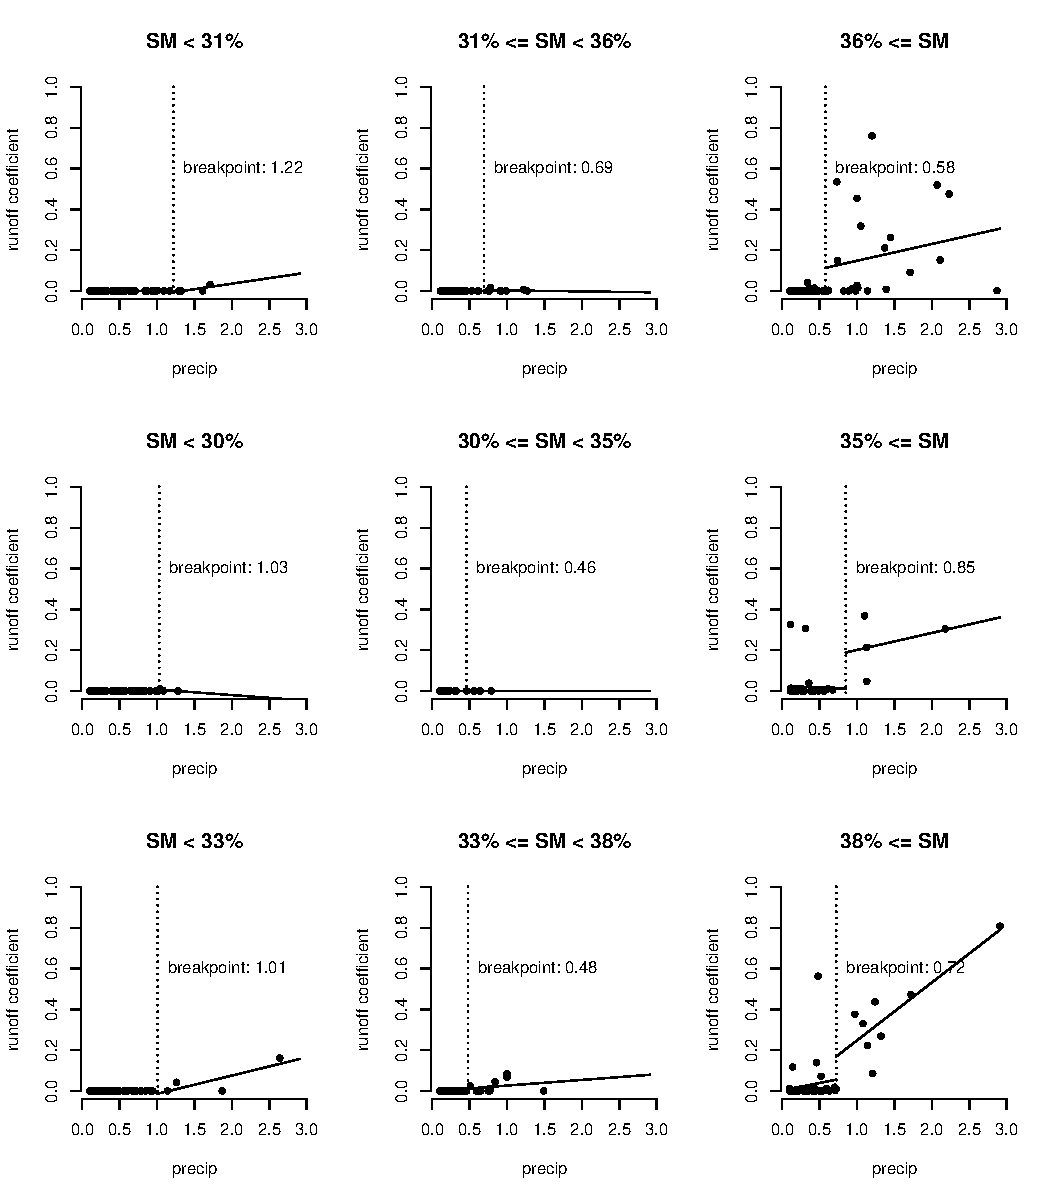
\includegraphics{runoff-precip_binned}
    \end{center}
    \caption{Top row: Koepke, middle row: Pagel, bottom row: Saxon.\label{precip_binned}}
\end{figure}


Rather than three bins, let's try two (above vs. below the SM breakpoint):\\


\begin{Schunk}
\begin{Soutput}
Intensity breakpoints at koepke when binned by soil moisture:
-Inf <= SM < 35: 1.9
35 <= SM < Inf: 1.6

Intensity breakpoints at pagel when binned by soil moisture:
-Inf <= SM < 35: 1.3
35 <= SM < Inf: 0.6

Intensity breakpoints at saxon when binned by soil moisture:
-Inf <= SM < 40: 0.9
40 <= SM < Inf: 2
\end{Soutput}
\end{Schunk}



\begin{figure}
    \begin{center}
\includegraphics{runoff-I30_binned2}
    \end{center}
    \caption{Top row: Koepke, middle row: Pagel, bottom row: Saxon.\label{I30_binned2}}
\end{figure}


When we put the events in bins based on their antecedent soil moisture (SM: high or low), the following are the precipitation breakpoints (units are centimeters of rain):\\

\begin{Schunk}
\begin{Soutput}
Precipitation breakpoints at koepke when binned by soil moisture:
-Inf <= SM < 35: 1.97
35 <= SM < Inf: 1.58

Precipitation breakpoints at pagel when binned by soil moisture:
-Inf <= SM < 35: 2.62
35 <= SM < Inf: 2.03

Precipitation breakpoints at saxon when binned by soil moisture:
-Inf <= SM < 40: 2.01
40 <= SM < Inf: 2.26
\end{Soutput}
\end{Schunk}



\begin{Schunk}
\begin{Sinput}
>     anova.bp <- function(data, split.on, site=NA, conts=FALSE, discrete.xrange=FALSE, xrange=NA, min.in.node=4, return.models=FALSE, return.X=FALSE)
+     {       
+         if(!conts)
+         {
+             if(discrete.xrange)
+                 th <- which.min( sapply(X=xrange, FUN=piecewise_disjoint, x=data[data$site==site,split.on], y=data[data$site==site,]$rc) ) + xrange[1]-1
+             else
+             {
+                 lower_lim = sort( data[data$site==site,split.on] )[min.in.node]
+                 upper_lim = sort(data[data$site==site,split.on], decreasing=T )[min.in.node]
+                 th <- optimize(piecewise_disjoint, upper=upper_lim, lower=lower_lim, x=data[data$site==site,split.on], y=data[data$site==site,]$rc)$minimum
+             }
+         
+             X.bp = cbind( ifelse(data[data$site==site,split.on]>=th, 1, 0), data[data$site==site,split.on], pmax(0, data[data$site==site,split.on]-th) )
+         }
+         else
+         {
+             if(discrete.xrange)
+                 th <- which.min( sapply(X=xrange, FUN=piecewise_conts, x=data[data$site==site,split.on], y=data[data$site==site,]$rc) ) + xrange[1]-1
+             else
+             {
+                 lower_lim = sort( data[data$site==site,split.on] )[min.in.node]
+                 upper_lim = sort(data[data$site==site,split.on], decreasing=T )[min.in.node]
+                 th <- optimize(piecewise_conts, upper=upper_lim, lower=lower_lim, x=data[data$site==site,split.on], y=data[data$site==site,]$rc)$minimum
+             }
+         
+             X.bp = cbind( data[data$site==site,split.on], pmax(0, data[data$site==site,split.on]-th) )   
+         }
+             
+         X.line = data[data$site==site,split.on]
+         y = data[data$site==site,]$rc
+        
+         if(return.X)
+             return(list(line=X.line, bp=X.bp, theta=th))
+         
+         fit.bp = lm(y~X.bp)
+         fit.line = lm(y~X.line)
+         
+         if(return.models)
+             return(list(bp=fit.bp, line=fit.line, theta=th))
+         
+         cat(paste("theta= ", th, "\n", sep=""))
+         
+         if(!conts)
+             1-pf(q=(sum(fit.line$resid**2) - sum(fit.bp$resid**2)) / 3 / (sum(fit.bp$resid**2)/(length(fit.bp$resid)-5)), df1=3, df2=length(fit.bp$resid)-5)
+         else
+             1-pf(q=(sum(fit.line$resid**2) - sum(fit.bp$resid**2)) / 2 / (sum(fit.bp$resid**2)/(length(fit.bp$resid)-4)), df1=3, df2=length(fit.bp$resid)-4)
+     }
\end{Sinput}
\end{Schunk}


\begin{figure}
    \begin{center}
\includegraphics{runoff-precip_binned2}
    \end{center}
    \caption{Top row: Koepke, middle row: Pagel, bottom row: Saxon.\label{precip_binned2}}
\end{figure}

\end{document}
